\section{Virtual Machines Preparation}

\centeredlargetext{white}{black}{
Virtual Machines Preparation
}

\begin{frame}
\frametitle{Virtual Machines Preparation}
\begin{itemize}
\item Get USB Memory Stick
\pause
\item Install VirtualBox from it
\pause
\item Import the VirtualMachine file
\pause
\item Boot the Virtual Machine
\pause
\item Log in
\pause
\item Get familiar with directories
\end{itemize}
\end{frame}


\begin{frame}
\frametitle{USB Memory Stick Content}
\framesubtitle{Directories and Files}
\begin{itemize}
\item VirtualBoxInstallers
\begin{itemize}
\item VirtualBox-4.0.8-71778-OSX.dmg (Mac)
\item VirtualBox-4.0.8-71778-Win.exe (Windows)
\item (Ubuntu Linux)
\begin{itemize}
\item virtualbox-4.0\_4.0.8-71778~Ubuntu~lucid\_amd64.deb
\item virtualbox-4.0\_4.0.8-71778~Ubuntu~lucid\_i386.deb
\item virtualbox-4.0\_4.0.8-71778~Ubuntu~maverick\_amd64.deb
\item virtualbox-4.0\_4.0.8-71778~Ubuntu~maverick\_i386.deb
\item virtualbox-4.0\_4.0.8-71778~Ubuntu~natty\_amd64.deb
\item virtualbox-4.0\_4.0.8-71778~Ubuntu~natty\_i386.deb
\item \ldots
\end{itemize}
\end{itemize}
\pause
\item VirtualMachine
\begin{itemize}
\item  "{859d59f9-ed19-4aa2-9cd6-a852ba47cdac}.vmdk"
\item  "OpenCV-ITK.ovf"
\end{itemize}
\end{itemize}
\end{frame}

\begin{frame}
\frametitle{Copy content in plain directories}
\begin{itemize}
\item LUIS to do this once the VM is ready.
\item The same source trees should be in plain dirs in the USB memory stick
\end{itemize}
\end{frame}

\begin{frame}
\frametitle{Install VirtualBox}
\begin{itemize}
\item Select the installer for your platform
\item Run it
\end{itemize}
\end{frame}

\begin{frame}
\frametitle{Alternative Linux Installation}
\begin{itemize}
\item  You can also install VirtualBox by doing:
\item  sudo apt-get install virtualbox-ose-qt
\end{itemize}
\end{frame}

\begin{frame}
\frametitle{Importing the Virtual Machine}
\begin{itemize}
\item Run VirtualBox
\item In ``File'' Menu select ``Import Appliance''
\item Provide the filename in the USB stick "VirtualMachine/OpenCV-ITK.ovf"
\item A progress bar will appear, and when it finishes you should see:
\end{itemize}
\begin{center}
  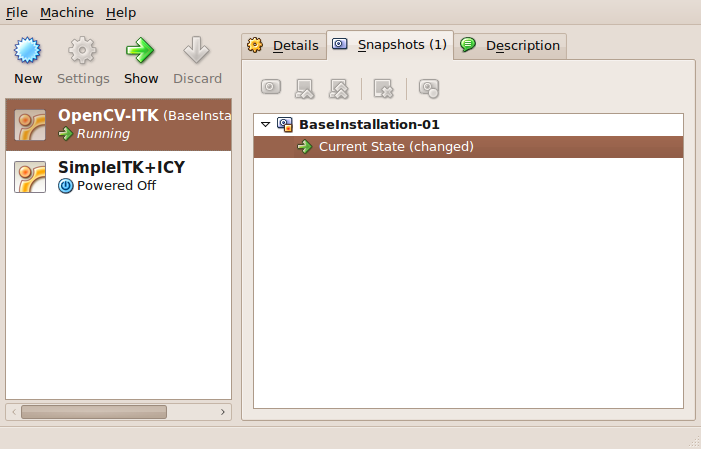
\includegraphics[width=0.5\paperwidth]{Screenshot-VirtualBox-OSE-01.png}
\end{center}
\end{frame}

\begin{frame}
\frametitle{Booting the Virtual Machine}
\begin{itemize}
\item Click on the ``OpenCV-ITK'' icon on the left, to select it.
\item Click on the Green Arrow at the top ``Show''.
\item The VM will start to boot and you will see the warning:
\end{itemize}
\begin{center}
  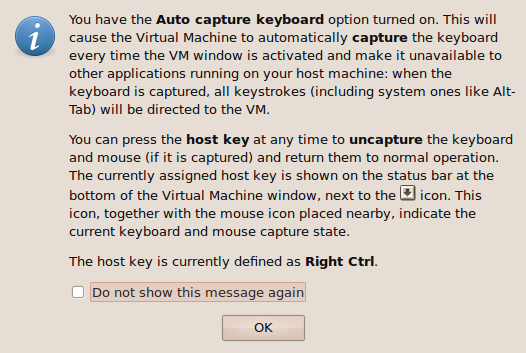
\includegraphics[width=0.4\paperwidth]{Screenshot-VirtualBox-OSE-02.png}
\end{center}
\begin{itemize}
\item Click ``OK''
\end{itemize}
\end{frame}

\begin{frame}
\frametitle{Booting the Virtual Machine}
\begin{itemize}
\item The boot sequence should continue and you shold see:
\end{itemize}
\begin{center}
  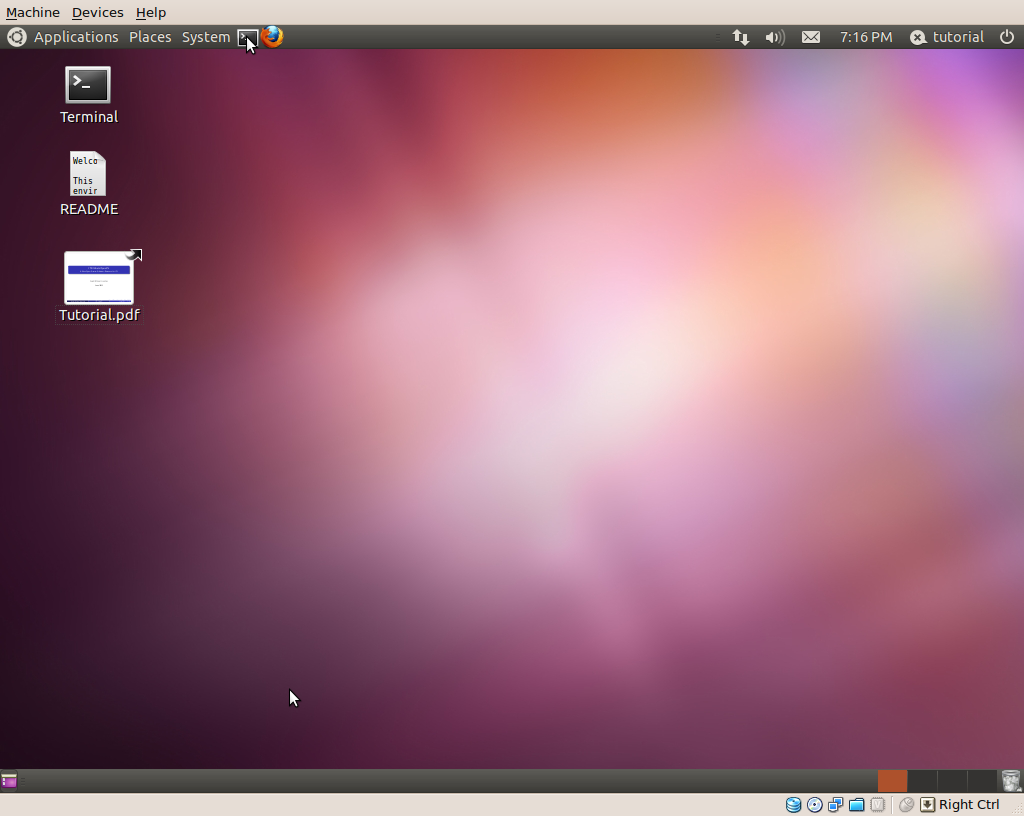
\includegraphics[width=0.7\paperwidth]{Screenshot-OpenCV-ITK-VirtualBox-01.png}
\end{center}
\end{frame}

\centeredlargetext{white}{black}{
Your Virtual Machine is Ready !
}
